\section{Principal Queries}

In this section we propose some queries to access our database:

\begin{enumerate}
	\item Find the most rented models, i.e. the cars that were rented above the average.
	\item Find the best performing branch in terms of total income from sales.
	\item Find the best-selling car model.
	\item For each kind of replacement part, find the supplier which supplies it at lowest cost.
\end{enumerate}

\begin{lstlisting}[language=SQL,
keywordstyle=\color{blue},
stringstyle=\color{mauve},
showstringspaces=false,
basicstyle=\ttfamily\footnotesize]
SELECT Model.name, COUNT(*) AS num_rent
FROM Model
JOIN Car ON Model.name = Car.name
JOIN Rental ON Car.lp = Rental.lp
GROUP BY Model.name
HAVING COUNT(*) > (SELECT AVG(num_rent)
    FROM (SELECT COUNT(*) AS num_rent
    FROM Model
    JOIN Car ON Model.name = Car.name
    JOIN Rental ON Car.lp = Rental.lp
    GROUP BY Model.name) AS foo);
\end{lstlisting}

\begin{center}
	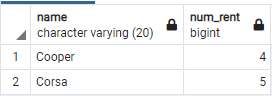
\includegraphics[scale=0.75]{1query.png}
\end{center}

\begin{lstlisting}[language=SQL,
keywordstyle=\color{blue},
stringstyle=\color{mauve},
showstringspaces=false,
basicstyle=\ttfamily\footnotesize]

SELECT branchid, SUM(total_sales) AS total_sales_branch FROM
    (SELECT employee, SUM(price) AS total_sales
    FROM Sale
    GROUP BY employee
    ORDER BY total_sales DESC) AS T FULL JOIN Employee AS E
    ON T.employee = E.tc
GROUP BY branchid
ORDER BY total_sales_branch DESC;
\end{lstlisting}

\begin{center}
	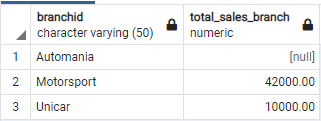
\includegraphics[scale=0.75]{2query.png}
\end{center}

\begin{lstlisting}[language=SQL,
keywordstyle=\color{blue},
stringstyle=\color{mauve},
showstringspaces=false,
basicstyle=\ttfamily\footnotesize]
SELECT model, num
FROM (  SELECT c.name AS model, count(*) AS num
        FROM car AS c INNER JOIN sale AS s ON c.lp = s.lp
        GROUP BY c.name ) AS counter1
WHERE num = (
        SELECT max(num)
        FROM (  SELECT c.name AS model, count(*) AS num
                FROM car AS c INNER JOIN sale AS s ON c.lp = s.lp
                GROUP BY c.name ) AS counter2 );
\end{lstlisting}

\begin{center}
	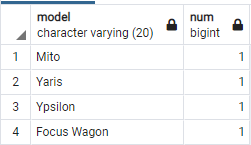
\includegraphics[scale=0.75]{3query.png}
\end{center}

\begin{lstlisting}[language=SQL,
keywordstyle=\color{blue},
stringstyle=\color{mauve},
showstringspaces=false,
basicstyle=\ttfamily\footnotesize]
SELECT s.supplier, p.category, MIN(s.catalog_price)
FROM supplies AS s INNER JOIN partkind AS p ON p.name = s.partkind
GROUP BY s.supplier, p.category
ORDER BY s.supplier ASC;
\end{lstlisting}

\begin{center}
	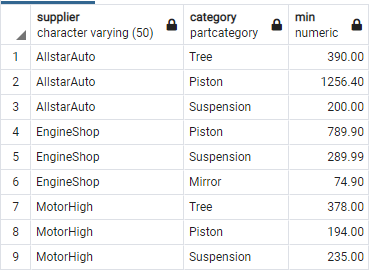
\includegraphics[scale=0.75]{4query.png}
\end{center}
